% IEEE conference template (IEEEtran, conference mode), as in
% https://www.overleaf.com/latex/templates/ieee-conference-template/grfzhhncsfqn
\documentclass[conference]{IEEEtran}
\IEEEoverridecommandlockouts
\usepackage{cite}
\usepackage{amsmath,amssymb,amsfonts}
\usepackage{algorithm}
\usepackage{algorithmic}
\usepackage{graphicx}
\usepackage{textcomp}
\usepackage{xcolor}
\usepackage{booktabs}
\usepackage{url}
\usepackage{tikz}
\usetikzlibrary{arrows.meta,positioning,calc,fit}
\def\BibTeX{{\rm B\kern-.05em{\sc i\kern-.025em b}\kern-.08em
    T\kern-.1667em\lower.7ex\hbox{E}\kern-.125emX}}

\newcommand{\R}{\mathbb{R}}
\newcommand{\T}{^{\top}}
\newcommand{\mpc}{\mathrm{MPC}}
\newcommand{\xb}{\bar{x}}
\newcommand{\ub}{\bar{u}}
\newcommand{\zb}{\bar{z}}
\newcommand{\lb}{\bar{\lambda}}
\newcommand{\xh}{\hat{x}}
\DeclareMathOperator*{\argmin}{arg\,min}
\renewcommand{\algorithmicrequire}{\textbf{Input:}}
\renewcommand{\algorithmicensure}{\textbf{Output:}}

\begin{document}

\title{Where Should the Residual Go? Residual Reinforcement Learning over Whole-Body Model Predictive Control for Humanoid Locomotion%
\thanks{Progress report. This work is carried out under the supervision of Prof.~Fumio Kanehiro and Dr.~Mehdi Benallegue.}}

\author{\IEEEauthorblockN{Norawit Nangsue}
% TODO(author): complete the affiliation and e-mail before submitting.
\IEEEauthorblockA{[Affiliation to be completed]}}

\maketitle

\begin{abstract}
Model predictive control (MPC) gives a humanoid robot a plan that respects its dynamics and constraints, but only as well as its model allows.
Reinforcement learning (RL) improves from experience, but it does not expose a plan and gives no constraint guarantee.
Residual RL adds a learned correction to the MPC output and is a natural way to combine the two.
This report asks where that correction should enter.
We describe three injection points of increasing structure: the controller output, the feedback policy returned by differential dynamic programming, and the optimality conditions of the MPC problem itself.
For the first, we show that the plan the MPC publishes is no longer the motion the robot will execute once a residual is added, and we give a residual-aware preview that restores it, together with a low-cost approximation based on Riccati gains and a safety gate that falls back to the residual-free plan.
For the second and third, we give low-dimensional parametrizations that keep the correction consistent with the solver's local model.
As the base controller for all three, we implemented an intrinsically stable MPC gait generator with a reformulated footstep timing and position pre-optimization, feeding a whole-body MPC of the HRP-5P legs.
In MuJoCo simulation it walks at up to 0.3\,m/s with a mean whole-body solve time of 6.7\,ms, and recovers from 26 of 36 pushes.
Its failures, which are mostly lateral pushes and contact moments that the sole cannot transmit, define what the residual policy has to learn.
No residual policy has been trained yet; the experiments are specified but not run.
\end{abstract}

\begin{IEEEkeywords}
humanoid robots, legged locomotion, model predictive control, residual reinforcement learning, safety filter
\end{IEEEkeywords}

% ======================================================================================================
\section{Introduction}

Two families of controllers now make humanoid robots walk.
The model-based family plans with a model: a reduced model such as the linear inverted pendulum (LIPM) \cite{kajita2001lipm,kajita2003preview} decides where the centre of mass (CoM) and the feet should go, and a whole-body controller, increasingly a whole-body MPC \cite{tassa2012synthesis,mastalli2020crocoddyl,dantec2022wbmpc}, turns that into joint torques.
The learning family trains a neural network policy in simulation with RL and transfers it to the robot \cite{hwangbo2019learning,lee2020learning,rudin2022minutes,radosavovic2024humanoid}.

Their strengths are complementary.
An MPC handles constraints explicitly, can be re-targeted without retraining, and publishes its plan, so an operator or a supervisor can inspect what the robot is about to do.
Its solution is optimal only for its model, and the model leaves out joint flexibility, contact compliance, actuator dynamics and the terms dropped to make the problem solvable in real time.
An RL policy absorbs such effects from experience and is robust in practice, but it is a black box: it gives no plan, no constraint guarantee, and its behaviour is set at training time.

Residual RL \cite{silver2018residual,johannink2019residual} keeps the model-based controller and learns only a correction that is added to its output.
The base controller makes exploration start from a working behaviour, and the policy only has to learn what the model misses.
Recent legged-robot results follow this pattern or a close variant \cite{gangapurwala2022rloc,kang2023rlmodel,jenelten2024dtc,cheng2025rambo,jeon2025residualmpc}.

Adding a correction at the output is the simplest choice, but not the only one, and it has a cost that is easy to overlook: \emph{once the residual is added, the plan published by the MPC is no longer the motion that will be executed.}
The properties that motivated keeping the MPC, namely a plan that can be previewed and constraints that are known to hold, are then lost exactly where the residual acts.
This report studies that problem and two alternatives that avoid it by injecting the residual deeper into the controller.

The contributions of this progress report are:
\begin{itemize}
\item A base controller for the study (Section~\ref{sec:base}): an IS-MPC gait generator \cite{scianca2020ismpc} with footstep timing and position pre-optimization \cite{dallard2025adios}, for which we propose a scaled reformulation solved as a single nonlinear program, feeding a whole-body MPC of the HRP-5P \cite{kaneko2019hrp5p} legs built on Crocoddyl \cite{mastalli2020crocoddyl}.
\item An analysis of three residual injection points (Section~\ref{sec:residual}): the output, the feedback policy, and the optimality conditions, with a common view of what each one preserves.
\item For the output residual, a residual-aware preview, a Riccati-gain approximation that needs no additional MPC solve, and a safety gate with a residual-free fallback.
\item Preliminary simulation results of the base controller (Section~\ref{sec:results}) that quantify its limits, and an experimental plan (Section~\ref{sec:plan}).
\end{itemize}

% ======================================================================================================
\section{Related Work}

\subsection{Gait generation with reduced models}
The zero-moment point (ZMP) \cite{vukobratovic2004zmp} and the LIPM \cite{kajita2001lipm} are the basis of preview control \cite{kajita2003preview} and of linear MPC gait generators, which later included the footsteps among the decision variables \cite{wieber2006mpc,herdt2010online}.
The unstable part of the LIPM is the divergent component of motion (DCM), also called the capture point \cite{pratt2006capture,takenaka2009dcm,englsberger2011capture}; capturability analysis \cite{koolen2012capturability} relates it to the number of steps needed to stop.
Lanari \emph{et al.} \cite{lanari2014boundedness} gave the condition under which the CoM stays bounded, and IS-MPC \cite{scianca2020ismpc} enforces this condition as a constraint.
Dallard \emph{et al.} \cite{dallard2025adios} closed the loop on the measured state and added a pre-optimization of footstep timing and position, as timing adaptation is essential for push recovery \cite{khadiv2020timing}.
Our base controller follows this line and the open-source implementation \cite{ismpcwalking}.

\subsection{Whole-body MPC}
Differential dynamic programming (DDP) \cite{mayne1966ddp} and iLQR \cite{li2004ilqr} solve the whole-body optimal control problem fast enough for MPC \cite{tassa2012synthesis,mastalli2020crocoddyl}, and have been demonstrated on a torque-controlled humanoid \cite{dantec2022wbmpc}.
A property that matters here is that the backward pass returns time-varying feedback gains with the trajectory.
These Riccati gains are a first-order approximation of how the MPC solution changes with the state, and they are used to run the feedback at a higher rate than the solver \cite{grandia2019feedback,dantec2022firstorder}.

\subsection{Reinforcement learning and its combination with MPC}
Policies trained with massively parallel simulation \cite{rudin2022minutes} and PPO \cite{schulman2017ppo} are now standard for legged robots \cite{hwangbo2019learning,lee2020learning,radosavovic2024humanoid}.
Model-based controllers enter this pipeline in several ways.
The policy can be asked to track a model-based plan, as in DTC \cite{jenelten2024dtc} or in on-demand optimal control references \cite{kang2023rlmodel}; it can output corrections to a model-based controller, as in RLOC \cite{gangapurwala2022rloc}, RAMBO \cite{cheng2025rambo} and Residual MPC \cite{jeon2025residualmpc}, the last of which adds torque residuals to a GPU-parallel whole-body MPC on a humanoid; or the MPC can be distilled into a network \cite{carius2020mpcnet,reske2021imitation}, which is fast but discards the online constraint handling.
A different approach places the optimization inside the learner, by differentiating through it \cite{amos2017optnet,amos2018diffmpc,romero2024acmpc} or by treating the MPC as a parametrized policy and value function \cite{gros2020nmpcrl}; gains and cost weights have also been learned directly \cite{buchli2011variable,marco2016lqr}.
In contrast to these works, we compare where the residual enters the same controller and what happens to the published plan in each case.
Policies that output a short sequence of future actions \cite{zhao2023act,chi2023diffusion} share our motivation for a preview, but they do not relate it to a model.

\subsection{Safety filters}
A safety filter lets an arbitrary policy act unless a model predicts a constraint violation \cite{alshiekh2018shielding,ames2019cbf,hewing2020lbmpc,brunke2022safe}.
The predictive safety filter \cite{wabersich2021psf} solves an MPC problem to find the closest safe input; \emph{gatekeeper} \cite{agrawal2024gatekeeper} instead forward-simulates a candidate followed by a backup trajectory and commits to it only if the whole trajectory is valid.
On legged robots, filters have mostly used reduced models, with full-order filters appearing recently \cite{nguyen2024gameplay}.
Our gate follows the gatekeeper pattern with the residual-free MPC plan as the backup.

\subsection{Model mismatch in optimization}
In process control, modifier adaptation \cite{marchetti2009modifier} corrects a model-based optimum by adding first-order terms to the cost and constraints, so that the modified problem has the optimality conditions of the real plant.
It builds on the sensitivity analysis of nonlinear programs \cite{fiacco1983sensitivity}.
The third injection point of Section~\ref{sec:residual} is a learned form of this idea.

% ======================================================================================================
\section{Base Controller}
\label{sec:base}

\begin{figure*}[t]
\centering
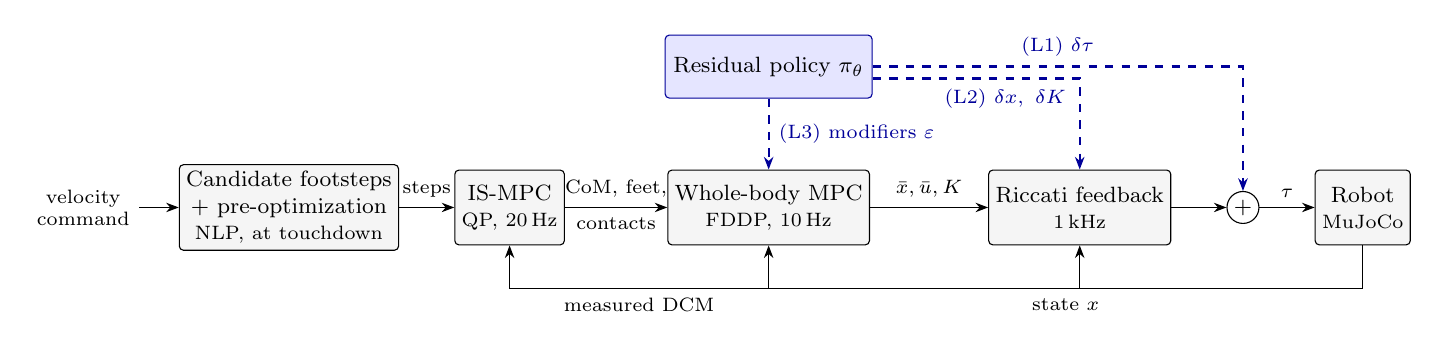
\begin{tikzpicture}[font=\footnotesize, >={Stealth[length=1.6mm]},
  blk/.style={draw, rounded corners=1.5pt, minimum height=9.5mm, align=center, inner sep=2.5pt, fill=black!4},
  res/.style={draw, rounded corners=1.5pt, minimum height=8mm, align=center, inner sep=3pt, fill=blue!10, draw=blue!60!black},
  lab/.style={font=\scriptsize, align=center},
  inj/.style={->, dashed, blue!60!black, thick}]
\node[lab] (cmd) {velocity\\command};
\node[blk, right=5mm of cmd] (ftpp) {Candidate footsteps\\+ pre-optimization\\{\scriptsize NLP, at touchdown}};
\node[blk, right=7mm of ftpp] (ismpc) {IS-MPC\\{\scriptsize QP, 20\,Hz}};
\node[blk, right=13mm of ismpc] (wb) {Whole-body MPC\\{\scriptsize FDDP, 10\,Hz}};
\node[blk, right=15mm of wb] (ric) {Riccati feedback\\{\scriptsize 1\,kHz}};
\node[circle, draw, inner sep=1pt, right=7mm of ric] (sum) {$+$};
\node[blk, right=7mm of sum] (rob) {Robot\\{\scriptsize MuJoCo}};
\draw[->] (cmd) -- (ftpp);
\draw[->] (ftpp) -- node[lab, above] {steps} (ismpc);
\draw[->] (ismpc) -- node[lab, above] {CoM, feet,} node[lab, below] {contacts} (wb);
\draw[->] (wb) -- node[lab, above] {$\xb,\ub,K$} (ric);
\draw[->] (ric) -- (sum);
\draw[->] (sum) -- node[lab, above] {$\tau$} (rob);
\coordinate (fb) at ($(rob.south)+(0,-5.5mm)$);
\draw[->] (rob.south) -- (fb) -| node[lab, pos=0.25, below] {state $x$} (wb.south);
\draw[->] (fb -| ric.south) -- (ric.south);
\draw[->] (fb -| wb.south) -| node[lab, pos=0.25, below] {measured DCM} (ismpc.south);
\node[res, above=9mm of wb] (pol) {Residual policy $\pi_\theta$};
\draw[inj] (pol.east) -| node[lab, pos=0.25, above, text=blue!60!black] {(L1) $\delta\tau$} (sum.north);
\draw[inj] (pol.east) ++(0,-1.5mm) -| node[lab, pos=0.32, below, text=blue!60!black] {(L2) $\delta x,\ \delta K$} (ric.north);
\draw[inj] (pol.south) -- node[lab, right, text=blue!60!black] {(L3) modifiers $\varepsilon$} (wb.north);
\end{tikzpicture}
\caption{Base controller (grey) and the three residual injection points studied in this report (blue, dashed): (L1) at the controller output, (L2) in the feedback policy returned by the DDP solver, (L3) in the optimality conditions of the whole-body MPC. Only the base controller is implemented so far.}
\label{fig:arch}
\end{figure*}

Fig.~\ref{fig:arch} shows the controller.
A gait generator based on the LIPM runs at 20\,Hz and produces CoM, foot and contact references; a whole-body MPC of the legs tracks them at 10\,Hz; its feedback policy is evaluated at 1\,kHz.

\subsection{LIPM and the stability condition}
With CoM position $c\in\R^2$, ZMP $p$ and $\eta=\sqrt{g/z_c}$ for a constant CoM height $z_c$, the LIPM is $\ddot c=\eta^2(c-p)$.
The DCM $\xi=c+\dot c/\eta$ splits it into a stable and an unstable first-order system,
\begin{equation}
\dot c=\eta(\xi-c),\qquad \dot\xi=\eta(\xi-p).
\label{eq:dcm}
\end{equation}
The CoM follows the DCM, and the DCM diverges from the ZMP.
The DCM stays bounded if and only if \cite{lanari2014boundedness}
\begin{equation}
\xi(t_0)=\eta\int_{0}^{\infty}e^{-\eta\tau}\,p(t_0+\tau)\,d\tau .
\label{eq:stab}
\end{equation}
The initial DCM cannot be chosen, so \eqref{eq:stab} is a constraint on the future ZMP trajectory.
IS-MPC \cite{scianca2020ismpc} enforces it while keeping the ZMP in the support polygon, by moving both the ZMP and the footsteps.

\subsection{Footstep timing and position pre-optimization}
After a push, \eqref{eq:stab} may have no solution with the nominal step times.
The pre-optimization of \cite{dallard2025adios} therefore adjusts the step positions $p_f^k$ and times $t_k$ before the MPC runs.
If the ZMP stays in the support region for all future times, integrating \eqref{eq:stab} piecewise over the steps shows that the initial DCM must lie in a time-weighted sum of the support regions.
With $\mu_k=e^{-\eta t_k}$ and $\Delta\mu_k=\mu_k-\mu_{k+1}$, the centre and half-size of this set are
\begin{equation}
c_\mu=\sum_{k=0}^{N_s-1}p_f^k\,\Delta\mu_k+p_f^{\mathrm{end}}\mu_{N_s},\quad
h_\mu=\sum_{k=0}^{N_s-1}\tfrac{d_k}{2}\,\Delta\mu_k+\tfrac{d}{2}\mu_{N_s},
\label{eq:ch}
\end{equation}
and the condition reads, in the frame $R$ of the support foot,
\begin{equation}
-h_\mu\le R\T\big(\xi(t_0)-c_\mu\big)+s\le h_\mu ,
\label{eq:ftpp}
\end{equation}
with a slack $s$ that is zero when the condition can be met.
Double support is sampled with the region moving linearly between the two feet, and all footsteps after the current one use the square inscribed in the sole ($d_k=d_y/\sqrt2$), so that \eqref{eq:ftpp} does not depend on their orientation.
Kinematic limits bound each step relative to the previous one, and timing constraints keep the phases ordered and within minimum and maximum durations.

The cost of \cite{dallard2025adios} penalizes the deviation from the nominal timing, the slack, and the footstep displacement weighted by a ratio of the form $(\Delta\mu_i)^2/(\Delta\hat\mu_i)^2$, where the hat denotes nominal values.
Two points make this problem awkward.
The variables $\mu_k$ decay exponentially with time and reach $10^{-7}$ at the end of a 5\,s preview, so the problem is badly scaled.
The reference implementation \cite{ismpcwalking} solves it by block coordinate descent, alternating twice between positions and times with a QP solver, and drops the divisor of the ratio.

We replace the decision variable $\mu_k$ by the ratio $\nu_k=\mu_k/\hat\mu_k$, which equals one when the timing is nominal.
The cost becomes
\begin{multline}
J=\sum_k(\nu_k-1)^2+w_s\|s\|^2\\
+K_s\sum_{i\ge1}\big\|p_f^i-\hat p_f^i\big\|^2\,
\frac{(\nu_i\hat\mu_i-\nu_{i-1}\hat\mu_{i-1})^2}{(\hat\mu_i-\hat\mu_{i-1})^2},
\label{eq:cost}
\end{multline}
all variables are of order one, and the ratio is kept as in the original formulation.
We solve positions and times jointly as one nonlinear program with CasADi \cite{andersson2019casadi} and IPOPT \cite{wachter2006ipopt}.
The program is built once per number of steps and cached, with the state, candidates and nominal timing as parameters, so a replan only runs the solver.

\subsection{IS-MPC}
The QP of IS-MPC takes the pre-optimized steps as candidates.
Its variables are the ZMP velocities $\dot p_j$ over a control horizon $T_c=2.5$\,s sampled at $\delta=50$\,ms and the footstep positions in that horizon.
It minimizes
\begin{equation}
\sum_j\|\dot p_j\|^2+\beta\sum_k\|p_f^k-\hat p_f^k\|^2+\gamma\sum_j\|p_j-\sigma_j\|^2 ,
\end{equation}
where $\sigma_j$ is the centre of the support region at sample $j$, subject to the ZMP lying in the (moving) support region, the kinematic limits, and the discrete form of \eqref{eq:stab},
\begin{equation}
\sum_{j=0}^{N_t-1}e^{-j\eta\delta}\dot p_j+\mathrm{tail}(p_f)=\frac{\eta}{1-e^{-\eta\delta}}\big(\xi_0-p_0\big).
\label{eq:stabqp}
\end{equation}
The tail is the anticipative tail of \cite{scianca2020ismpc}: beyond $T_c$ the ZMP is conjectured to follow the remaining pre-optimized steps up to the preview horizon $T_p=6$\,s and to stop at the midpoint of the last two feet.
The centring term ($\gamma$) keeps the ZMP away from the sole edges and leaves the problem a convex QP because $\sigma_j$ is linear in the footsteps.
The QP is assembled directly as sparse matrices and solved with OSQP \cite{stellato2020osqp}.

The generator replans (pre-optimization and QP) at every touchdown and re-solves the QP with fixed steps at every 50\,ms tick.
It also contains a velocity gate, a two-step stop, capture steps when the DCM leaves the support region while standing, and a DCM feedback law for standing.
A push is detected when the difference between the measured and the planned DCM jumps by more than 4\,cm within one tick; the gait state is then reset to the measured one.
The whole gait generator is about 750 lines of Python.

\subsection{Whole-body MPC and its feedback policy}
\label{sec:wb}
The whole-body optimal control problem uses the floating base and the twelve leg joints of HRP-5P ($n_v=18$); the upper body is held by a separate joint-space LQR and inverse dynamics.
The horizon has $H=25$ nodes of 20\,ms.
Contacts are rigid 6D constraints that follow the contact schedule of the gait generator, and the cost tracks the CoM and foot references with posture and torque regularization.
The problem is solved with the FDDP solver of Crocoddyl \cite{mastalli2020crocoddyl}, using Pinocchio \cite{carpentier2019pinocchio} for the dynamics, every 100\,ms with at most ten warm-started iterations.

The solve at time $k$ returns the state and torque trajectories and the Riccati gains, $\{\xb_{i|k},\ub_{i|k},K_{i|k}\}_{i=0}^{H}$.
Between solves, the torque is
\begin{equation}
\tau=\ub_{i|k}+K_{i|k}\,(\xb_{i|k}\ominus x),
\label{eq:riccati}
\end{equation}
evaluated at 1\,kHz with the measured state $x$ and the plan interpolated in time; $\ominus$ is the difference on the state manifold.
We write $\tau^{\mpc}$ for \eqref{eq:riccati} in the following.

% ======================================================================================================
\section{Three Places for the Residual}
\label{sec:residual}

Let $\pi_\theta$ be the residual policy trained with RL to maximize a task return in the real system or in a high-fidelity simulation.
The working assumption of residual learning is that the optimal action for this return is close to the MPC action, so that a small correction is enough.
We state it as a bound relative to the size of the MPC action.
Let $\Delta^{\mpc}_k$ be the change commanded by the MPC at step $k$ and $\Delta^{\mathrm{res}}_k=\Delta^{\mpc}_k+\delta_k$ the change after the residual.
If $\|\delta_k\|\le\rho\,\|\Delta^{\mpc}_k\|$ with $\rho<1$, the two changes are aligned,
\begin{equation}
\frac{\Delta^{\mpc}_k\cdot\Delta^{\mathrm{res}}_k}{\|\Delta^{\mpc}_k\|\,\|\Delta^{\mathrm{res}}_k\|}\ \ge\ \sqrt{1-\rho^2}.
\label{eq:assump}
\end{equation}
The bound $\rho$ is a design parameter enforced by clipping the policy output.
Equation~\eqref{eq:assump} holds for the next step only.
Nothing similar holds for the steps after it, because the residuals accumulate through the dynamics; this is the subject of the next subsection.

\subsection{Level 1: residual at the controller output}
\label{sec:l1}
The simplest scheme adds the residual to the output,
\begin{equation}
\tau_k=\tau^{\mpc}_k+\delta\tau_k,\qquad \delta\tau_k=\pi_\theta\big(x_k,\mathcal P_k\big),
\label{eq:l1}
\end{equation}
where $\mathcal P_k=\{\xb_{i|k},\ub_{i|k}\}$ is the current plan, given to the policy as an observation.
For a robot under joint position control, the same scheme is written on the position target, $q^d_{k+1}=\bar q_{1|k}+\delta q_k$.
Training needs one MPC solve per control step, as in \cite{jeon2025residualmpc}.

\subsubsection{The published plan becomes invalid}
The MPC replans from the measured state at every cycle, so the executed action \eqref{eq:l1} never needs the future: the next solve already starts from the state the residual produced.
What is lost is the plan.
$\mathcal P_k$ was computed assuming $\delta\tau=0$ for the whole horizon.
Let $e_i=\xh_i\ominus\xb_{i|k}$ be the deviation of the motion that will really happen from the plan.
To first order,
\begin{equation}
e_{i+1}=A_ie_i+B_i\,\delta\tau_i ,
\label{eq:err}
\end{equation}
with $A_i,B_i$ the dynamics Jacobians along the plan.
A biped is open-loop unstable: by \eqref{eq:dcm}, the DCM component of $e_i$ grows as $e^{\eta t}$, a factor of 4.7 over our 0.5\,s horizon for $\eta=3.11$\,s$^{-1}$.
The plan is therefore reliable for the next step and progressively wrong after it.
This matters for two uses of the plan:
\begin{itemize}
\item \emph{Motion preview.} A supervisor, an operator display, or a higher-level planner that reads the plan sees a motion that will not be executed.
\item \emph{Future safety.} A step can satisfy every constraint now and still lead to a state from which no admissible motion exists, for example a DCM that can no longer be captured. Checking this requires the future motion with the residual included.
\end{itemize}

\subsubsection{Residual-aware preview}
To predict the motion at step $i>0$, the policy must be evaluated at the predicted state $\xh_i$, not at the current state, and the MPC term must be the one the MPC would output from $\xh_i$.
Algorithm~\ref{alg:preview} rolls the pair forward.
In the exact variant, the MPC is solved again at every predicted state.
The solves are sequential, since each needs the previous residual, but each is warm-started from the shifted previous solution.
We keep the horizon length constant and shift it, because a shrinking horizon is a different problem with different terminal effects; this requires references beyond the nominal horizon, which the gait generator provides since $T_c=2.5$\,s is five times the whole-body horizon.

\begin{algorithm}[t]
\caption{Residual-aware preview at time $k$}
\label{alg:preview}
\begin{algorithmic}[1]
\REQUIRE state $x_k$, plan $\{\xb_{i|k},\ub_{i|k},K_{i|k}\}$, policy $\pi_\theta$, model $f$, mode
\ENSURE predicted motion $\{\xh_i,\hat\tau_i\}_{i=0}^{N}$
\STATE $\xh_0\leftarrow x_k$;\quad $\mathcal P\leftarrow$ plan at time $k$
\FOR{$i=0$ \TO $N-1$}
  \IF{mode is \textsc{exact} \AND $i>0$}
    \STATE $\mathcal P\leftarrow$ solve the MPC from $\xh_i$, warm-started from $\mathcal P$
    \STATE $\tau^{\mpc}\leftarrow$ first torque of $\mathcal P$
  \ELSE
    \STATE $\tau^{\mpc}\leftarrow\ub_{i|k}+K_{i|k}(\xb_{i|k}\ominus\xh_i)$ \hfill\COMMENT{\textsc{riccati}}
  \ENDIF
  \STATE $\hat\tau_i\leftarrow\tau^{\mpc}+\pi_\theta(\xh_i,\mathcal P)$
  \STATE $\xh_{i+1}\leftarrow f(\xh_i,\hat\tau_i)$
\ENDFOR
\end{algorithmic}
\end{algorithm}

\subsubsection{Riccati preview}
The exact variant costs $N$ MPC solves per control step.
The Riccati gains give a cheaper alternative.
The policy $\ub_{i|k}+K_{i|k}(\xb_{i|k}\ominus x)$ is the first-order expansion of the MPC solution around the plan \cite{dantec2022firstorder}, so it approximates what a re-solved MPC would output from a nearby state.
The \textsc{riccati} mode of Algorithm~\ref{alg:preview} uses it in place of the solve.
The preview then costs $N$ policy inferences and $N$ model steps, with no additional solve, and the deviation follows the closed-loop version of \eqref{eq:err},
\begin{equation}
e_{i+1}=(A_i-B_iK_{i|k})\,e_i+B_i\,\delta\tau_i ,
\label{eq:errcl}
\end{equation}
which is contracting where \eqref{eq:err} was not.
The approximation is valid while the deviation is small and the contact sequence and active constraints do not change; the bound $\rho$ in \eqref{eq:assump} is what keeps the deviation small.
How far along the horizon it stays accurate is an empirical question (Experiment~2).

For a position-controlled robot, the preview is the same with $\xh_{i+1}=\xb_{i+1|i}+\delta x_i$, which assumes perfect tracking of the target; with torques, it is as good as the model $f$.
In both cases the preview is a model-based prediction of what the learned policy will do.
It does not predict the model error that the policy was trained to compensate.

\subsubsection{Safety gate}
With a preview, the residual can be gated.
The candidate trajectory applies the residual for the next step and the residual-free MPC afterwards; it is accepted if the predicted motion satisfies
\begin{equation}
g(\xh_i,\hat\tau_i)\le -m_i,\qquad i=0,\dots,N ,
\label{eq:gate}
\end{equation}
with margins $m_i$ that grow with $i$ to account for the prediction error.
Otherwise the controller executes $\tau^{\mpc}_k$ alone.
This is the gatekeeper pattern \cite{agrawal2024gatekeeper} with the MPC plan as the backup, and a discrete alternative to projecting the action onto the safe set \cite{wabersich2021psf}.
The checks we intend to use come from the base controller: joint and torque limits; the contact wrench cone, i.e., the centre of pressure inside the sole; and capturability, tested by solving the pre-optimization from the predicted DCM and requiring zero slack in \eqref{eq:ftpp}, which certifies that footsteps and timings satisfying \eqref{eq:stab} still exist.
The size of the correction made by the gate is penalized in the reward, so that the policy learns to stay inside it.

The guarantee is limited.
The gate ensures that the residual does not make the model-predicted motion worse than the base controller's.
It does not make the base controller safe, and Section~\ref{sec:results} shows that the base controller alone fails in some cases.

\subsection{Level 2: residual in the feedback policy}
\label{sec:l2}
The feedback law \eqref{eq:riccati} has two parts: a target $\xb$ and a reactiveness $K$.
Between two MPC solves, 100 control steps are executed with this law alone, and the residual policy can adjust both parts in that interval:
\begin{align}
\tau&=\ub+(K+\delta K)\,(\xb+\delta x\ominus x)\nonumber\\
&=\tau^{\mpc}+K\,\delta x+\delta K\,(\xb+\delta x\ominus x).
\label{eq:l2}
\end{align}

\emph{Target residual.} The term $K\delta x$ is a torque residual restricted to the range of $K$.
It is the response the MPC would give, to first order, if the state were displaced by $-\delta x$.
The policy thus acts as a learned bias on the state seen by the controller, and the torque that results respects the trade-offs encoded in the cost, which a free $\delta\tau$ does not.
The Riccati preview of Section~\ref{sec:l1} applies unchanged.

\emph{Gain residual.} The last term of \eqref{eq:l2} is bilinear: it has no effect without a tracking error, so it changes how the robot reacts to a disturbance and not the nominal motion.
A free $\delta K$ is not practical.
For the leg model, $K$ has $12\times36=432$ entries per node, and an arbitrary perturbation can destabilize the closed loop.
We consider two low-dimensional parametrizations.
(a)~Gain scaling per joint group, $K\leftarrow\mathrm{diag}(1+\alpha)K$ with bounded $\alpha$.
Continuous-time LQR tolerates a gain increase of any size and a reduction by half in each input channel when the input weight is diagonal \cite{safonov1977margins}; the margins of a discrete, time-varying, finite-horizon gain are smaller, so the bounds on $\alpha$ will be set empirically.
(b)~Cost residual: the policy outputs changes $\delta Q,\delta R$ of a few cost weights, and the backward pass is run again along the current trajectory.
The gains then remain optimal for the local model, at the cost of one backward pass, which is a fraction of a solver iteration.
This is related to variable impedance learning \cite{buchli2011variable} and to LQR weight tuning \cite{marco2016lqr}, applied here online to the gains of a whole-body MPC.

\subsection{Level 3: residual in the optimality conditions}
\label{sec:l3}
The deepest injection point is the optimization problem.
Write the MPC problem as $\min_z f(z)$ subject to $h(z)=0$, where $z$ collects states and controls and $h$ the dynamics and contact constraints.
Let $(\zb,\lb)$ be its solution, and let the real system have cost $f+\Delta f$ and constraints $h+\Delta h$ with solution $(z^\star,\lambda^\star)=(\zb+\delta z,\lb+\delta\lambda)$.
We assume: (A1) $\delta z$ is small; (A2) the set of active inequality constraints is the same for both problems, with strict complementarity, so that active inequalities can be treated as equalities and inactive ones ignored; (A3) the constraint gradients are linearly independent and the second-order sufficient condition holds, so the KKT matrix is invertible \cite{nocedal2006numerical}.

Expanding the KKT conditions of the real problem around $(\zb,\lb)$, the terms of the model problem cancel, and dropping second-order terms gives
\begin{equation}
\begin{bmatrix}\nabla^2\bar L&\partial\bar h\T\\ \partial\bar h&0\end{bmatrix}
\begin{bmatrix}\delta z\\ \delta\lambda\end{bmatrix}
=-\begin{bmatrix}r_s\\ r_p\end{bmatrix},
\label{eq:kkt}
\end{equation}
\begin{equation}
r_s=\nabla\Delta f(\zb)+\partial\Delta h(\zb)\T\lb,\qquad r_p=\Delta h(\zb),
\end{equation}
where $\bar L=f+\lb\T h$.
The correction to the whole trajectory is therefore \emph{the solver's own sensitivity applied to the mismatch}: the KKT matrix is known from the solver, and only the mismatch $(r_s,r_p)$ is unknown.
$r_p$ is the constraint violation of the model solution in the real system, in particular the one-step prediction error of the dynamics, and can be measured from rollouts; $r_s$ is a gradient mismatch that has to be learned.

At Level~3, the policy outputs the mismatch and the solver computes the correction.
In practice the mismatch is injected as modifiers $\varepsilon=(\varepsilon_s,\varepsilon_p)$ of the problem,
\begin{equation}
\min_z\ f(z)+\varepsilon_s\T z\quad\text{s.t.}\quad h(z)+\varepsilon_p=0 ,
\label{eq:modified}
\end{equation}
whose first-order optimality conditions coincide with \eqref{eq:kkt}.
This is modifier adaptation \cite{marchetti2009modifier}, with the modifiers given by a policy as a function of the state instead of an iterative update at a steady operating point.
In a DDP solver, $\varepsilon_p$ is a bias on the dynamics of each node and $\varepsilon_s$ a linear cost term, such as a shift of the CoM or foot reference; both are available in Crocoddyl without changing the solver.
The action dimension is set by the basis chosen for $\varepsilon$ and can be small.

This level has three properties that Level~1 lacks.
The corrected trajectory satisfies the model constraints because the solver enforces them.
The Riccati gains are those of the corrected problem.
The published plan already includes the correction, so the preview problem of Section~\ref{sec:l1} does not arise.
Unlike differentiable MPC \cite{amos2018diffmpc,romero2024acmpc} or MPC-parametrized RL \cite{gros2020nmpcrl}, no derivative of the solver is needed: the solver is part of the environment and the policy is trained with a standard policy-gradient method.

Assumption (A2) is the weak point for a legged robot, since the active set changes at every contact switch.
We will hold the modifiers constant within a contact phase and define the basis per phase.

\subsection{Summary}
Table~\ref{tab:levels} compares the three levels.
All of them produce a torque correction; they differ in the set the correction is taken from.
At Level~1 it is arbitrary; at Level~2 it lies in the range of the Riccati gains or modulates them; at Level~3 it is the solution of \eqref{eq:kkt} for the whole horizon.
Moving from Level~1 to Level~3 trades expressiveness for consistency with the model, and we expect the appropriate level to depend on how large and how structured the model error is.

\begin{table}[t]
\caption{The three residual injection points}
\label{tab:levels}
\centering
\setlength{\tabcolsep}{3.5pt}
\resizebox{\columnwidth}{!}{%
\begin{tabular}{@{}lccc@{}}
\toprule
 & L1: output & L2: feedback & L3: optimality\\
\midrule
Policy output & $\delta\tau$ or $\delta q^d$ & $\delta x$; $\alpha$ or $\delta Q,\delta R$ & modifiers $\varepsilon$\\
Correction set & unrestricted & range of $K$, gains & solution of \eqref{eq:kkt}\\
Model constraints & not enforced & first order & enforced\\
Published plan & invalid & valid to first order & valid\\
Extra cost per step & none$^{\mathrm a}$ & $\le$ one backward pass & none\\
Main risk & unsafe actions & gain instability & active-set change\\
\bottomrule
\multicolumn{4}{@{}l}{$^{\mathrm a}$The preview costs $N$ solves (exact) or $N$ model steps (Riccati).}
\end{tabular}}
\end{table}

% ======================================================================================================
\section{Preliminary Results: Base Controller}
\label{sec:results}

No residual policy has been trained.
This section reports the base controller alone, to establish the baseline and to identify what the residual has to correct.

\subsection{Setup}
The HRP-5P model (59 degrees of freedom including the floating base, 104\,kg) is simulated in MuJoCo \cite{todorov2012mujoco} with a 1\,ms time step and torque control.
The LIPM height is the measured CoM height when the MPC starts ($z_c=1.014$\,m, $\eta=3.11$\,s$^{-1}$).
Steps last at most 0.8\,s, of which 85\,\% is single support, and the commands are limited to 0.3\,m/s forward and 0.3\,rad/s.
All runs are headless, on one thread of a laptop (Apple M5), with the controller computed inside the simulation loop, so computation time does not delay the control.
A run counts as a fall when the base drops below 0.5\,m.
Pushes are applied as an instantaneous change of the base velocity, $\Delta v=\eta\,d$, which shifts the DCM by $d$; for example, $d=0.08$\,m is 0.25\,m/s, an impulse of about 26\,N\,s.

\subsection{Walking}
Table~\ref{tab:walk} summarizes four commands, each applied for 5\,s (8\,s in the last row) and followed by a two-step stop.
The robot does not fall in any of them, and Fig.~\ref{fig:walk} shows the 0.3\,m/s run.
The measured DCM follows the planned one with an RMS error of 12 to 16\,mm, and the feet track their references within 31\,mm.
The whole-body solve takes 6.7\,ms on average and at most 14.2\,ms of the 100\,ms period, with 8.2 iterations on average.
A gait tick takes 2.2\,ms on average; a touchdown replan (pre-optimization and QP) takes 7.2\,ms on average and at most 11.9\,ms.
The first replan from standing takes 49\,ms, just within the 50\,ms tick.

\begin{table}[t]
\caption{Walking in simulation (base controller, no falls)}
\label{tab:walk}
\centering
\setlength{\tabcolsep}{3pt}
\resizebox{\columnwidth}{!}{%
\begin{tabular}{@{}lcccccc@{}}
\toprule
Command & Dist. & Steps & \multicolumn{2}{c}{Error (max) [mm]} & CoP & Solve [ms]\\
 & [m] & & foot & DCM & ratio$^{\mathrm a}$ & mean / max\\
\midrule
0.2\,m/s & 0.93 & 8 & 18 & 28 & 1.45 & 6.4 / 14.2\\
0.3\,m/s, 0.2\,rad/s & 1.46 & 9 & 31 & 40 & 1.81 & 6.9 / 10.0\\
$-0.15$\,m/s & 0.74 & 8 & 10 & 30 & 1.47 & 6.1 / 8.7\\
0.3\,m/s (8\,s) & 2.43 & 13 & 30 & 36 & 1.59 & 7.1 / 11.6\\
\bottomrule
\multicolumn{7}{@{}l}{$^{\mathrm a}$Largest measured CoP offset of a stance foot divided by the half-size}\\
\multicolumn{7}{@{}l}{\phantom{$^{\mathrm a}$}of the largest centred box inside the sole; above 1 is near the sole edge.}
\end{tabular}}
\end{table}

\begin{figure}[t]
\centering
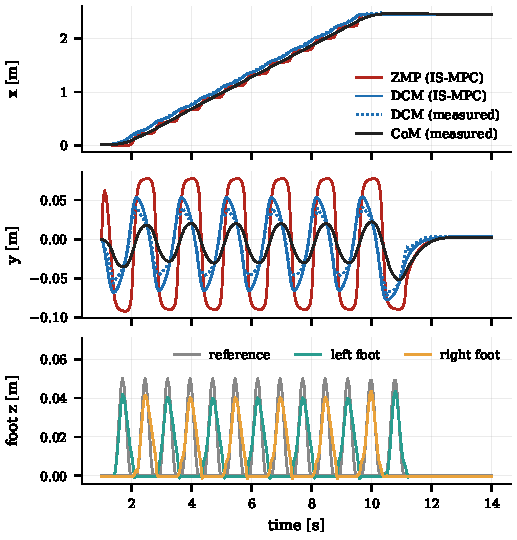
\includegraphics[width=\columnwidth]{figures/walk.pdf}
\caption{Walking at 0.3\,m/s for 8\,s, then stopping. Top and middle: ZMP and DCM planned by the IS-MPC, and DCM and CoM measured on the simulated robot. Bottom: foot height references and measured foot heights.}
\label{fig:walk}
\end{figure}

\subsection{Push recovery}
Table~\ref{tab:push} reports 36 pushes with the default settings: 20 while standing (five magnitudes, four directions) and 16 while walking at 0.2\,m/s (two magnitudes, four directions, two instants of the step cycle).
The robot stays up in 28 cases.
In two of them, lateral pushes of 0.10\,m while standing, it ends balanced on the edge of a foot tilted by 45$^\circ$, which we do not count as a recovery; this leaves 26 of 36.

\begin{table}[t]
\caption{Pushes survived, by DCM shift $d$ (four directions each)}
\label{tab:push}
\centering
\setlength{\tabcolsep}{4pt}
\begin{tabular}{@{}lcccccc@{}}
\toprule
\multicolumn{7}{@{}l}{\emph{Standing}}\\
$d$ [m] & 0.04 & 0.06 & 0.08 & 0.10 & 0.12 & Total\\
\midrule
Push detection on (default) & 4/4 & 4/4 & 4/4 & 1/4$^{\mathrm a}$ & 0/4 & 13/20\\
Push detection off & 4/4 & 4/4 & 2/4 & 1/4 & 0/4 & 11/20\\
\midrule
\multicolumn{7}{@{}l}{\emph{Walking at 0.2\,m/s} (two push instants)}\\
$d$ [m] & \multicolumn{2}{c}{0.05} & \multicolumn{2}{c}{0.08} & & Total\\
\midrule
Default & \multicolumn{2}{c}{7/8} & \multicolumn{2}{c}{6/8} & & 13/16\\
\bottomrule
\multicolumn{7}{@{}l}{$^{\mathrm a}$Two further cases stay up on a tilted foot and are not counted.}
\end{tabular}
\end{table}

\begin{figure}[t]
\centering
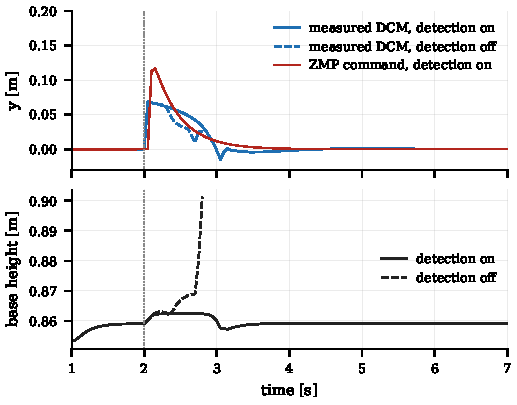
\includegraphics[width=\columnwidth]{figures/push.pdf}
\caption{Lateral push ($d=0.08$\,m, at 2\,s) while standing. With push detection, the gait state is reset to the measured DCM and the standing law moves the ZMP to bring it back. Without it, the whole-body MPC keeps tracking the unperturbed reference and the robot falls.}
\label{fig:push}
\end{figure}

Three observations follow.
First, closing the loop on the measured DCM helps while standing: with push detection, all pushes of 0.08\,m are recovered, against two of four without it (Fig.~\ref{fig:push}), and a forward push of 0.10\,m is recovered with a capture step.
Second, the failures are directional.
While walking, the three falls are all pushes toward the robot's right; while standing, the 0.10\,m failures are the backward push and the two lateral ones.
Third, in an earlier sweep with a previous parameter set, enabling push detection also during walking reduced the number of recovered pushes (17 of 24 against 21 of 24): resetting the reference to the pushed state removes the whole-body MPC's own pull toward the planned CoM.
Push detection is therefore active only while standing by default.

\subsection{What the residual has to correct}
The results point to three model errors.

\emph{Contact moments.} The CoP ratio in Table~\ref{tab:walk} exceeds 1 in every run, and after strong lateral pushes a stance foot rolls onto its edge.
The whole-body problem treats a stance foot as rigidly fixed, without a limit on the centre of pressure, so it plans ankle moments that the sole cannot transmit.
Adding a wrench-cone penalty to the cost was tried and made walking fail with every weight large enough to change the plan, because the problem relies on these moments to track the lateral CoM reference.

\emph{Mismatch between the two models.} The gait generator plans with the LIPM, and the robot lags its reference by 3 to 4\,cm of DCM in single support.
The interaction between the two loops is not captured by either model, as the third observation above shows.

\emph{Lateral recovery.} Lateral step limits are narrow ($\pm3.5$\,cm around the nominal foot separation), so lateral pushes are mostly handled by the ankle and by the whole-body motion, which the LIPM does not describe.

These are structured errors.
The first is a constraint missing from the model (a natural target for Level~3, where it enters as a modifier, or for the gate of Level~1); the second is a tracking lag (a target for Level~2); the third needs new behaviour outside the model (Level~1).

% ======================================================================================================
\section{Experimental Plan}
\label{sec:plan}

Table~\ref{tab:exp} lists the planned experiments.
The policy will be trained with PPO \cite{schulman2017ppo} in simulation, with pushes, mass and friction randomization and command changes, and compared with the base controller alone and with a policy trained without the MPC.
We plan to use mjlab \cite{zakka2026mjlab} so that training and the present MuJoCo evaluation share one physics engine.

\begin{table}[t]
\caption{Planned experiments}
\label{tab:exp}
\centering
\setlength{\tabcolsep}{3pt}
\begin{tabular}{@{}cp{0.36\columnwidth}p{0.47\columnwidth}@{}}
\toprule
 & Experiment & Question\\
\midrule
1 & L1, single MPC pass, position targets & Does a bounded output residual recover the failed pushes of Table~\ref{tab:push}?\\
2 & E1 + residual-aware preview (exact and Riccati) & How accurate is each preview along the horizon, and at what cost? The executed action equals E1.\\
3 & E1 and E2 with torque residuals & Does the preview hold when the future state comes from the model $f$?\\
4 & E2 + safety gate & How many violations are avoided, and how often does the gate intervene?\\
5 & MPC distilled into the policy & What is lost without the online MPC (baseline)?\\
6 & L2: target residual, gain scaling, cost residual & Does a structured residual match E1 with a smaller action space?\\
7 & L3: modifiers per contact phase & Does a residual in the optimality conditions keep the plan valid?\\
\bottomrule
\end{tabular}
\end{table}

\emph{Metrics.} Pushes survived on the protocol of Table~\ref{tab:push}; velocity tracking; DCM error; CoP ratio and constraint violations; preview error $\|\xh_i-x_{k+i}\|$ as a function of $i$; gate intervention rate; computation time.

\emph{Training cost.} The MPC runs on the CPU, so it bounds the training speed.
With the measured times, one simulated second costs about 67\,ms of whole-body solves and 44\,ms of gait ticks per environment.
At a 50\,Hz policy rate, $10^8$ policy steps are $2\times10^6$ simulated seconds, or about 60 core-hours of MPC, which is feasible on a CPU cluster without the GPU-parallel solver of \cite{jeon2025residualmpc}.
An exact preview in the training loop would multiply this by up to $H=25$.
For this reason the policy is trained in the single-pass setting of Experiment~1, and the preview and the gate are evaluated at deployment with the same policy; training with the gate in the loop is limited to the Riccati preview.

\emph{Open issues.} The whole-body MPC currently uses rigid contacts without a wrench cone; a formulation that walks with the cone active is needed before the gate can check it meaningfully.
The state is taken from the simulator, and an estimator is required for the robot.
The controller must then be ported to mc\_rtc for experiments on HRP-5P.

% ======================================================================================================
\section{Conclusion}
This report framed residual RL over MPC as a choice of where the learned correction enters the controller.
A residual at the output is the most expressive but invalidates the plan that the MPC publishes; we proposed a residual-aware preview, its Riccati approximation and a gate with a residual-free fallback to restore the preview and a limited form of safety.
A residual in the feedback policy or in the optimality conditions keeps the correction consistent with the solver's model, to first order or exactly, at the price of a restricted correction set.
The base controller needed for the study is implemented and walks in simulation; its measured failures give concrete targets for each level.
The next step is Experiment~1, followed by the comparison of the three levels on the same push protocol.

\bibliographystyle{IEEEtran}
\bibliography{refs}

\end{document}
